%--------------------------------------------------------%
% Figures
%--------------------------------------------------------%

%!TEX root = ../main.tex

%--------------------------------------------------------%
% DOCUMENT CLASS
%--------------------------------------------------------%

  % Change "letterpaper" to "a4" if you use a4 paper size
  \documentclass[letterpaper,12pt]{article}

%--------------------------------------------------------%
% TITLE SECTION
%--------------------------------------------------------%

  %Abstract
  \usepackage{abstract} % Allows abstract customization
  % Set the "Abstract" text to bold
  \renewcommand{\abstractnamefont}{\normalfont\bfseries}
  % Set the abstract itself to small italic text
  \renewcommand{\abstracttextfont}{\normalfont\small\itshape}

  %Title
  \usepackage{titlesec} % Allows customization of titles

  %Authors
  \usepackage{authblk} % For multiple authors

  %Date
  \usepackage{datetime} % allows for including today's date
  % These two lines creates a new date format ``Month day(th), year''
  \newdateformat{usvardate}{
  \monthname[\THEMONTH] \ordinal{DAY}, \THEYEAR}

%--------------------------------------------------------%
% HEADERS & FOOTERS
%--------------------------------------------------------%

  %Footnotes
  % \usepackage[bottom]{footmisc} % Makes footnotes stick to bottom of the page

  %Headers from page 2 on
  % \usepackage{fancyhdr}
  \pagestyle{plain}
  % \fancyheadoffset{0cm}
%   \setlength{\headheight}{15pt}

%--------------------------------------------------------%
% MACROS
%--------------------------------------------------------%

  % Define keywords macro command
  \providecommand{\keywords}[1]{\textbf{\textit{Keywords---}} #1}

%--------------------------------------------------------%
% MATH SUPPORT
%--------------------------------------------------------%

  % The amssymb package provides various useful mathematical symbols
  \usepackage{amssymb}
  % The amsthm package provides extended theorem environments
  \usepackage{amsthm}
  % The newtxmath package provides additional math symbol support
  % in Times New Roman symbols, etc.
  \usepackage{newtxmath}
  \usepackage{mathtools}
  \usepackage{blkarray, bigstrut}

%--------------------------------------------------------%
% FONTS
%--------------------------------------------------------%

  \usepackage{microtype} % Slightly tweak font spacing for aesthetics
  \usepackage[utf8]{inputenc}
  \usepackage{newtxtext} % Makes default font Adobe Times New Roman

%--------------------------------------------------------%
% LINES
%--------------------------------------------------------%

  % Spacing
  \usepackage{setspace} % See \doublespacing command at the top of content.tex
  % Numbering
  \usepackage{lineno} 	% See \linenumbers at the top of content.tex
  \usepackage[table,x11names]{xcolor}
  % Lists
  \usepackage{enumitem}
  \setlist{nosep}
  \setlist[itemize]{leftmargin=*}

%--------------------------------------------------------%
% MARGINS
%--------------------------------------------------------%

  %NOTE: All spaces in this template are in inches, because it is
  % formatted for letterpaper (8.5 x 11 inch) paper. If you use a4
  % paper, choose different sizes in millimeters or centimeters.
  \usepackage[top=1.5in, bottom=1.5in, left=1in, right=1in]{geometry}

%--------------------------------------------------------%
% COMMENTS
%--------------------------------------------------------%

  % \usepackage[colorinlistoftodos]{todonotes} % allows margin comments
  % See examples in content.tex, and here for manual:
  % http://www.ctan.org/pkg/todonotes
  \usepackage{soul} % allows for highlighting


%--------------------------------------------------------%
% ACRONYMS
%--------------------------------------------------------%

  \usepackage[nohyperlinks,nolist]{acronym} % Managing acronyms

%--------------------------------------------------------%
% GRAPHICS
%--------------------------------------------------------%

  \usepackage{graphicx,caption} % More advanced figure inclusion
  \graphicspath{{figures/}} % Set the default folder for images
  \usepackage{float} % For specifying table/figure locations, i.e. [ht!]

  % The printlen command allows the user to print the exact text width or height.
  % This is useful, when trying to create graphics (outside of LaTeX, of course)
  % with the optimal dimensions. See here for usage: http://www.ctan.org/pkg/printlen
  \usepackage{printlen}

  \usepackage[section]{placeins} % Used to ensure that figures do not go into the next section

%--------------------------------------------------------%
% TABLES
%--------------------------------------------------------%

  \usepackage{longtable} % For long tables that span multiple pages
  \newcommand{\sym}[1]{\rlap{#1}}% For symbols like *** in tables
  \usepackage{tabularx} % Allows advanced table features
  \newcolumntype{L}[1]{>{\raggedright\arraybackslash}p{#1}}
  \newcolumntype{C}[1]{>{\centering\arraybackslash}p{#1}}
  \newcolumntype{R}[1]{>{\raggedleft\arraybackslash}p{#1}}
  \usepackage{relsize} % Allows precise adjustment of font size,
  %useful for fitting tables to page width
  \usepackage{multirow}
  %for horizontal tables
  \usepackage{lscape}

%--------------------------------------------------------%
% REFERENCES
%--------------------------------------------------------%

  \usepackage{hyperref} % For hyperlinks in the PDF
  \usepackage{csquotes}
  \usepackage[style=nature,url=false,backend=biber,sorting=none]{biblatex}
  \bibliography{references/references.bib}


% \titleformat{\subsection}[runin]{}{}{}{}[]


\title{ \huge Inferring microbial co-occurrence networks from 16S data: A systematic evaluation }
\author{DK, GB, ZH, CD, KK, DS}
\date{\today}

\begin{document}

\maketitle

\begin{figure}[h]
  \centering
  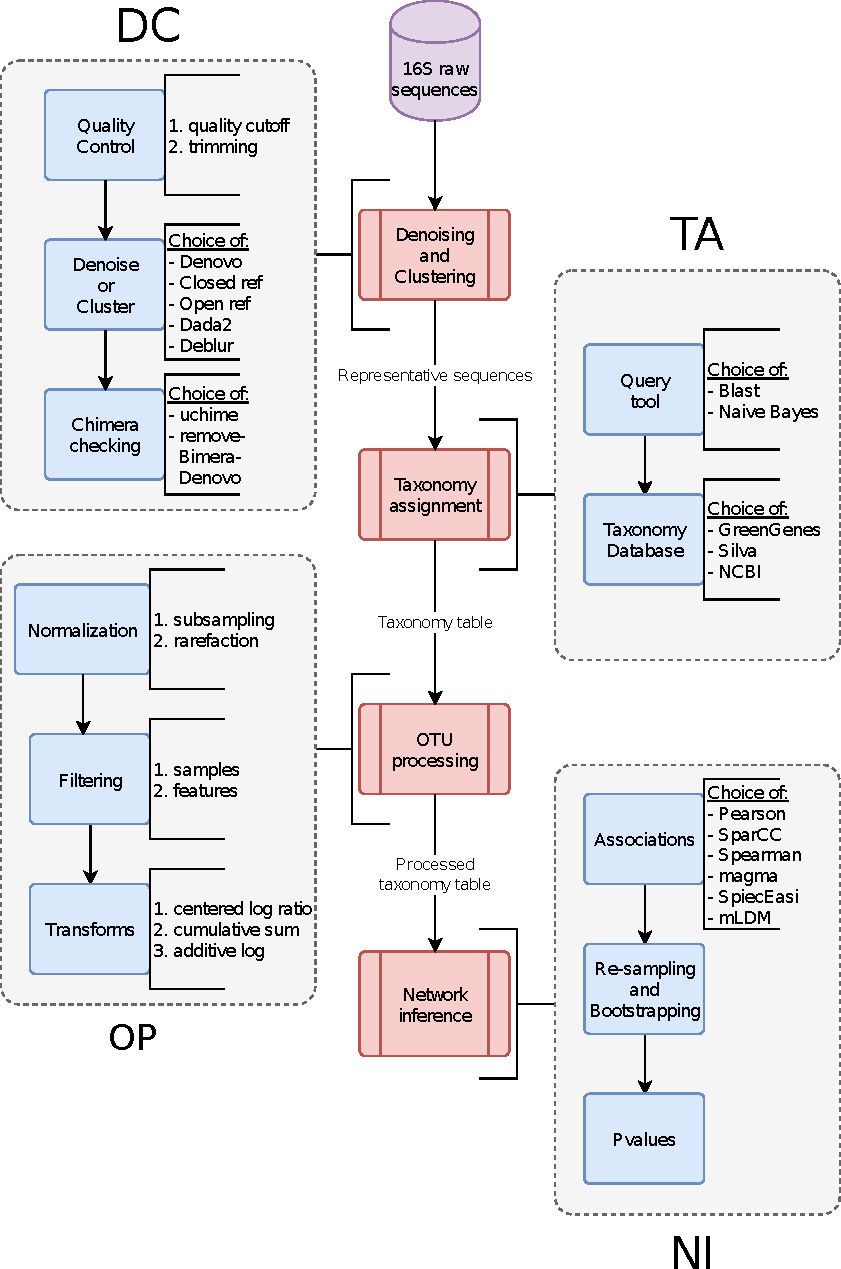
\includegraphics[width=0.67\linewidth]{figure1.pdf}
  \caption{
    \textbf{The workflow of the microbial co-occurrence analysis pipeline}.
    The processes can be grouped into four major steps: \textbf{(DC)} denoising and clustering, \textbf{(TA)} taxonomy assignment, \textbf{(OP)} OTU/ESV processing, and \textbf{(NI)} network inference.
    Each step incorporates several processes, each of which in turn have several alternate algorithms for the same task (indicated by the text to the right of the blue boxes).
    The text along the arrows describes the data that is being passed from one step to another.
  }
  \label{fig:figure1}
\end{figure}

\begin{figure}[h]
  \centering
  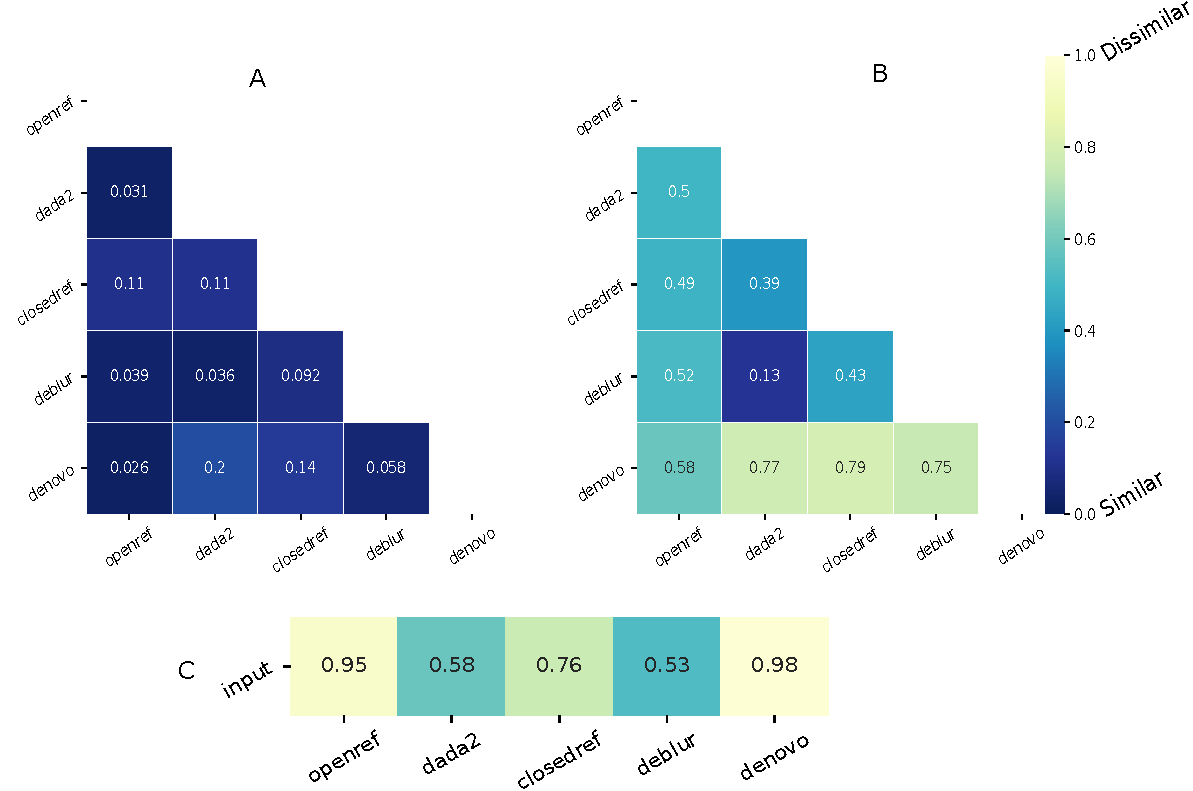
\includegraphics[width=0.75\linewidth]{figure2.pdf}
  \caption{
    \textbf{The choice of database contributes to the most variance in the networks}.
    \textbf{(A)} The relative variance in the networks contributed by the DC, TA and OP steps of the pipeline.
    \textbf{(B)} All combinations of inferred networks are shown as points on a PCA plot.
    The color of the points corresponds to the taxonomy database, the shape corresponds to the denoising/clustering method and the size corresponds to whether low abundance OTUs were removed or not.
    \textbf{(B inset)} The network generated using DC=dada2, TA=Greengenes, OP=off and NI=SPARCC and represents the particular point shown (green big triangle).
    The plot clearly shows that the points can be separated based on the TA step and that the differences due to the DC and OP steps are not as significant.
  }
  \label{fig:figure2}
\end{figure}

\begin{figure}[h]
  \centering
  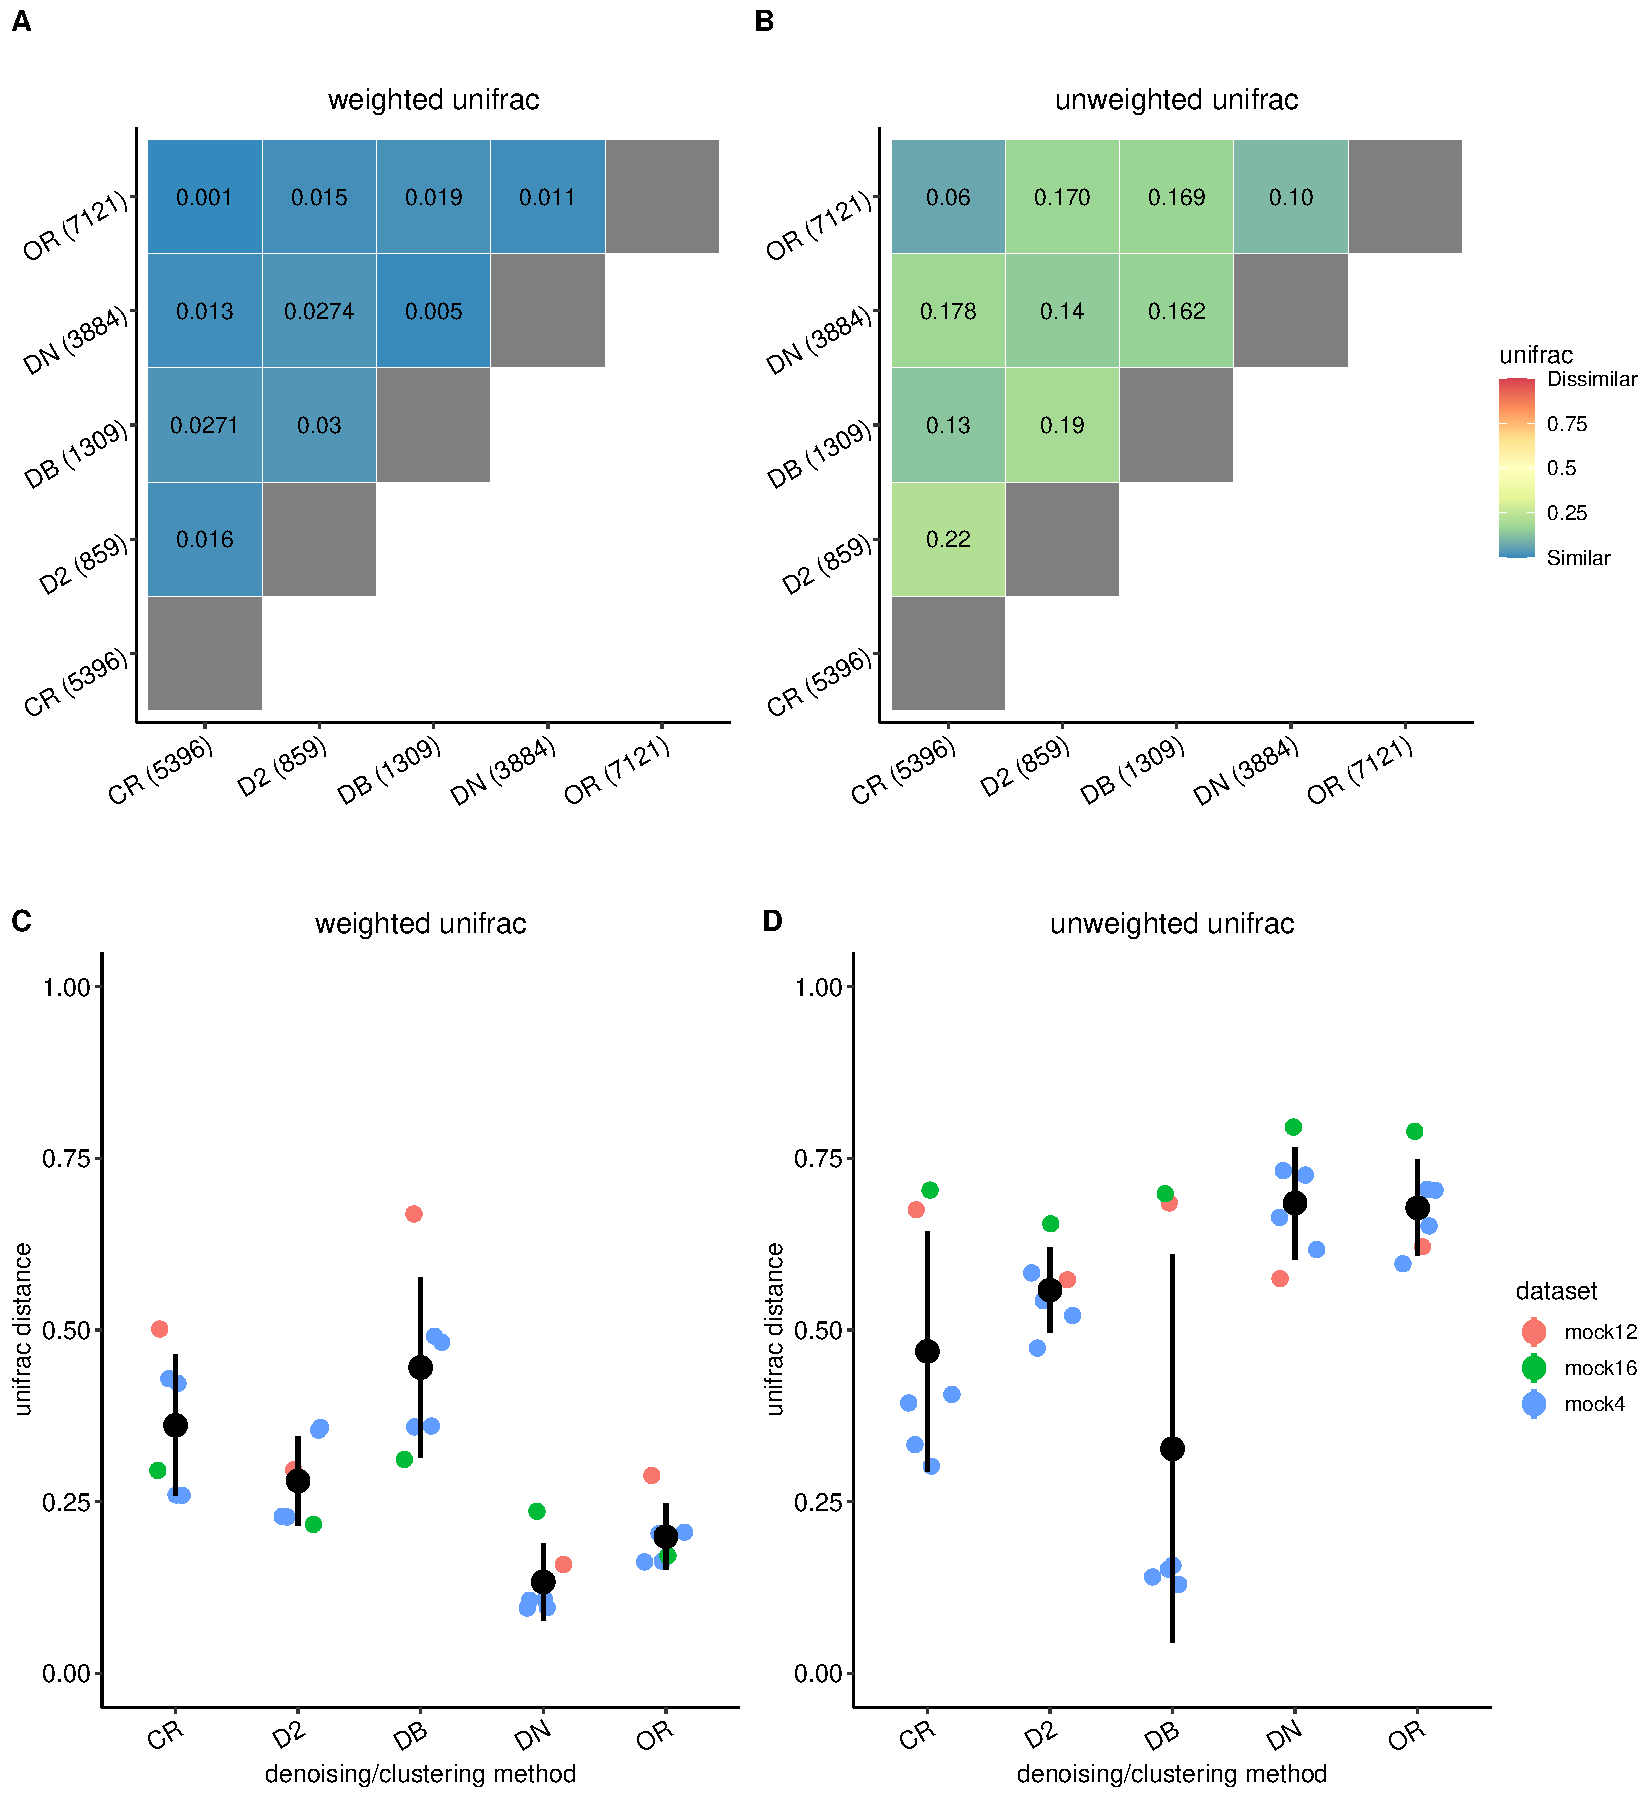
\includegraphics[width=0.8\linewidth]{figure3.pdf}
  \caption{
    \textbf{The representative sequences generated by the different denoising/clustering methods are very similar but differ slightly in the sequences that are in low abundance.}
    \textbf{(A)} The average weighted UniFrac distance between the representative sequences shows that the representative sequences and their compositions are fairly identical between the methods,
    \textbf{(B)} The relatively larger average unweighted UniFrac distance indicates that methods differ in their identification of sequences of low abundance,
    \textbf{(C)} The distributions of the average unweighted UniFrac distance between the expected sequence profile and the calculated sequence profile in mock datasets show that dada2 and Deblur were the best performing methods in most of the datasets.
  }
  \label{fig:figure3}
\end{figure}

\begin{figure}[h]
  \centering
  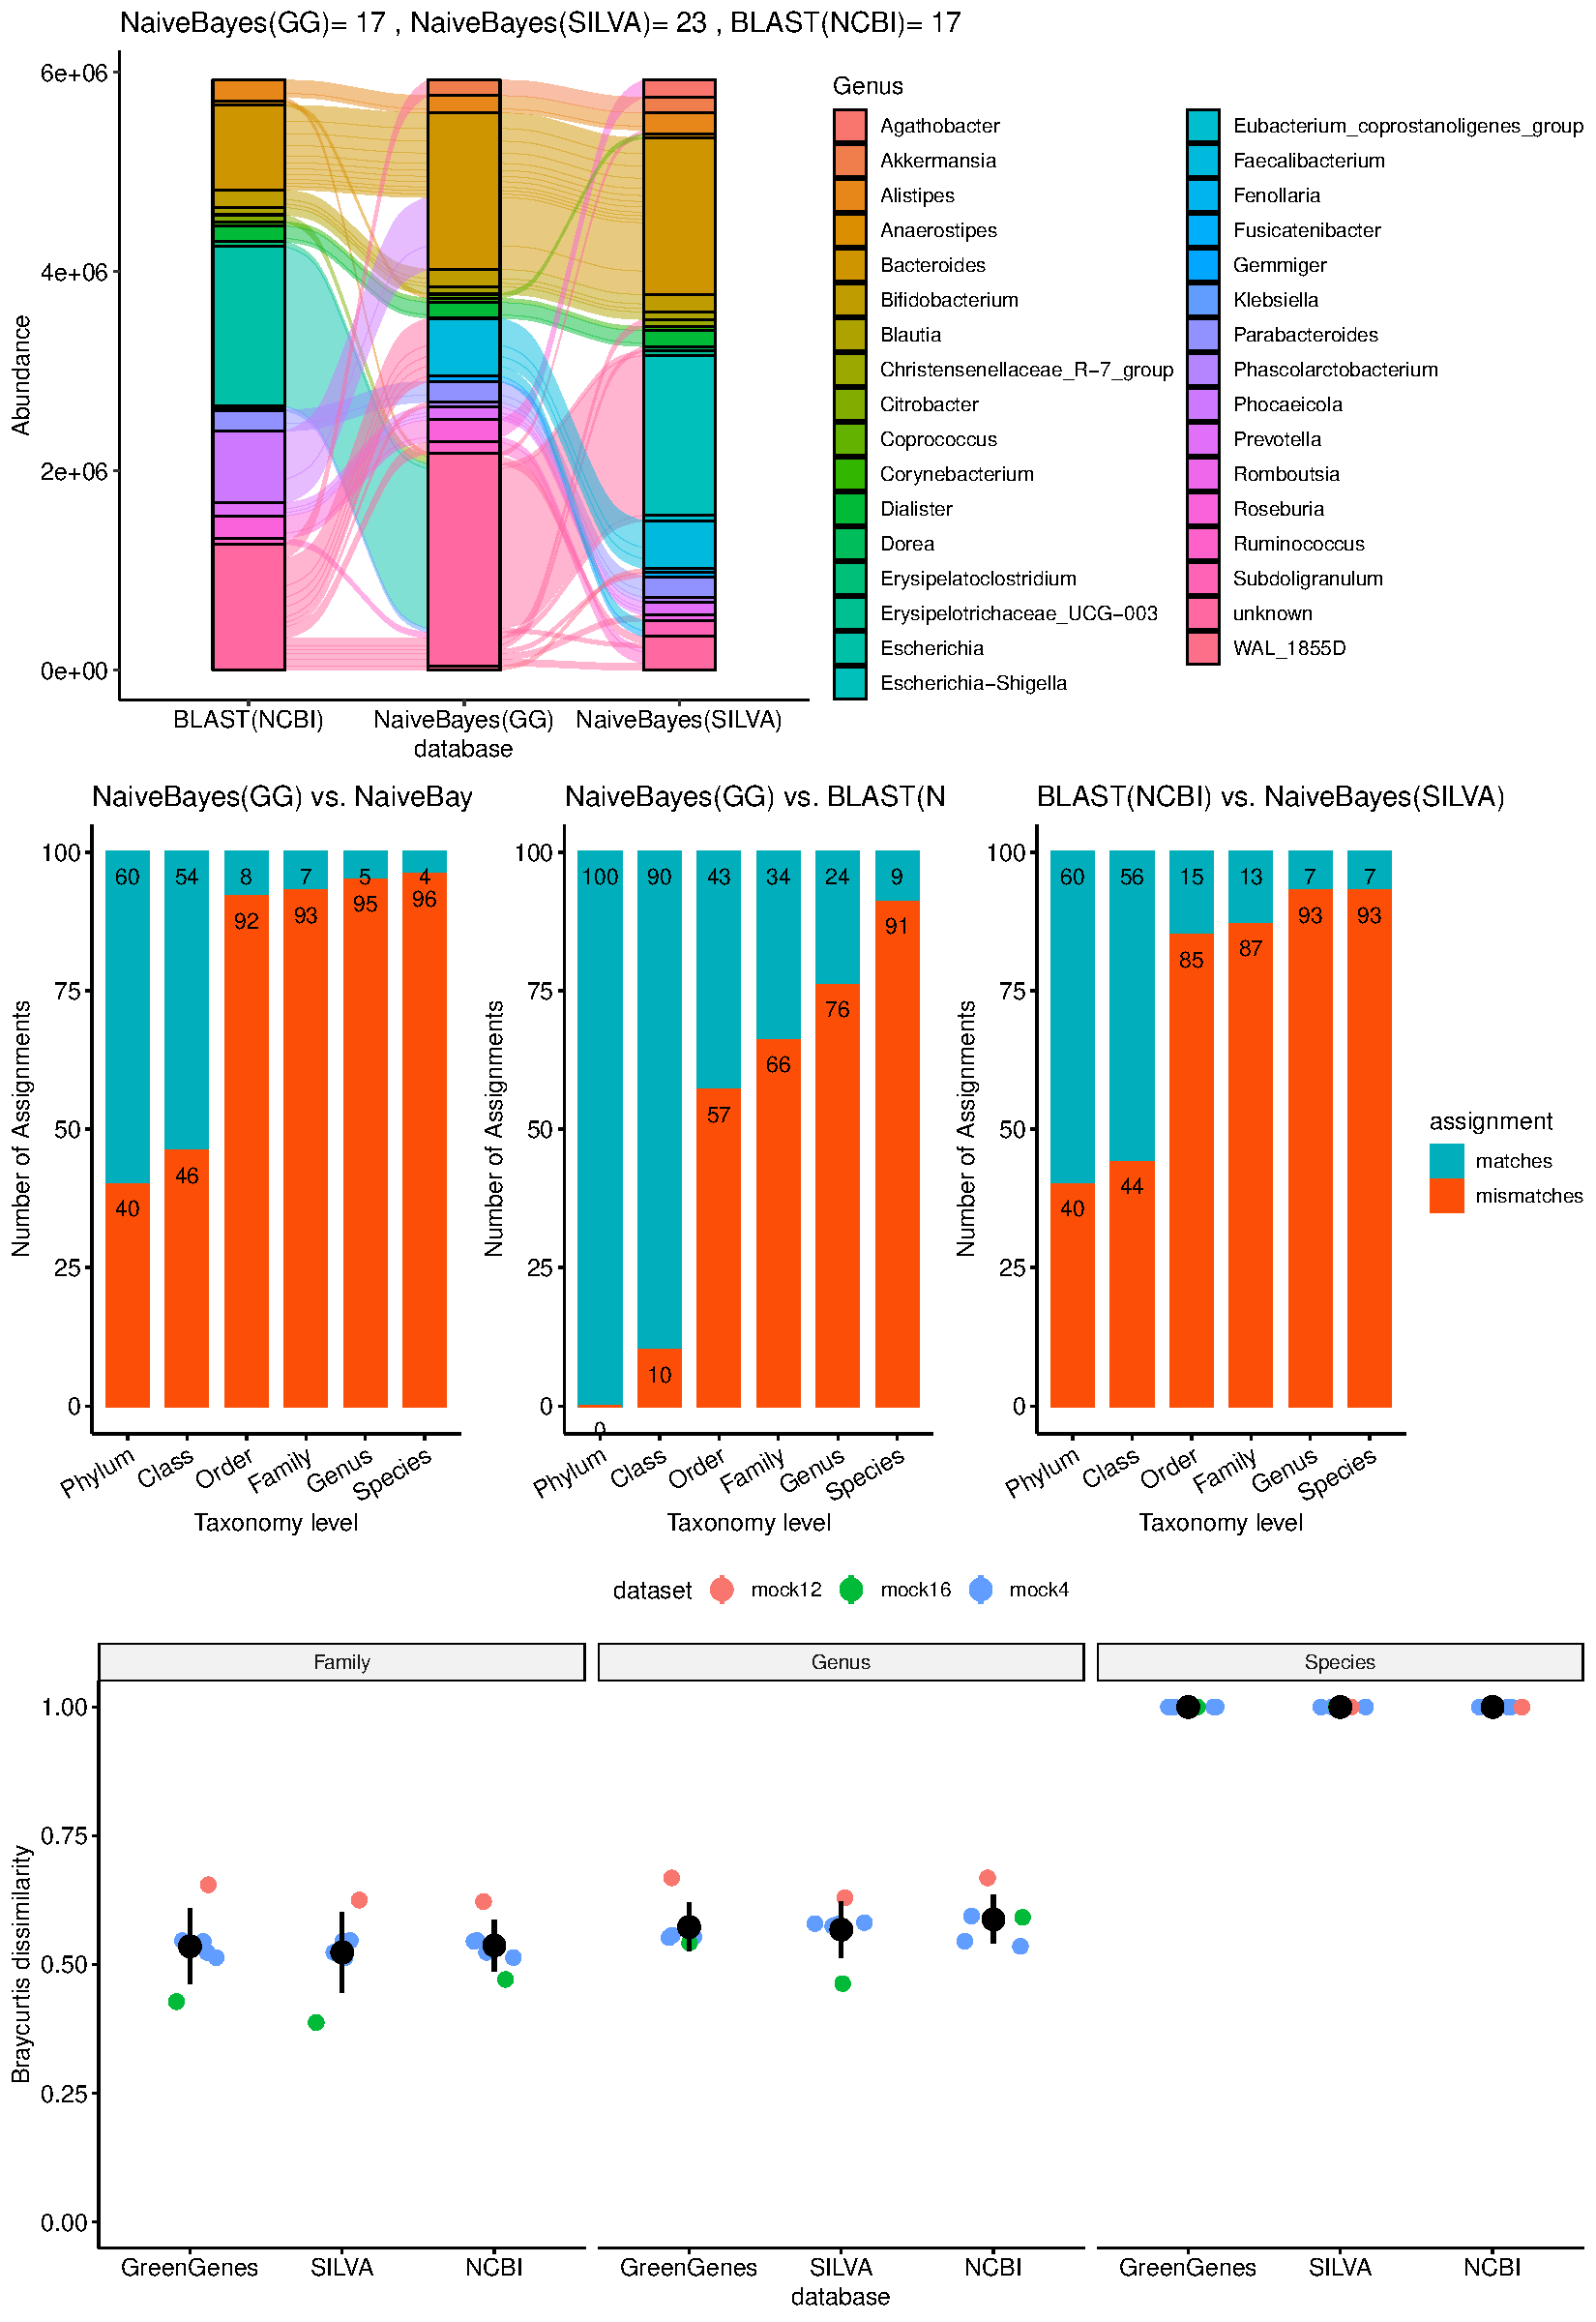
\includegraphics[width=0.75\linewidth]{figure4.pdf}
  \caption{
    \textbf{Taxonomic reference databases vary widely in terms of their taxonomies.}
    \textbf{(A)} The assignment of the top 50 representative sequences to their respective taxonomies using the three different reference databases shows how the same sequences are assigned to different genus.
    \textbf{(B)} The percentage of \ac{OTU}s assigned to the same taxonomic label when using different reference databases.
    The percentage of mismatches decrease at higher taxonomic levels but even at the Phylum level there exists around 10\% of mismatches.
    \textbf{(C)} The Bray-Curtis dissimilarity between the expected taxonomy profile and calculated taxonomy profile in the mock datasets shows that there is no best choice of database for every dataset.
  }
  \label{fig:figure4}
\end{figure}

\begin{figure}[h]
  \centering
  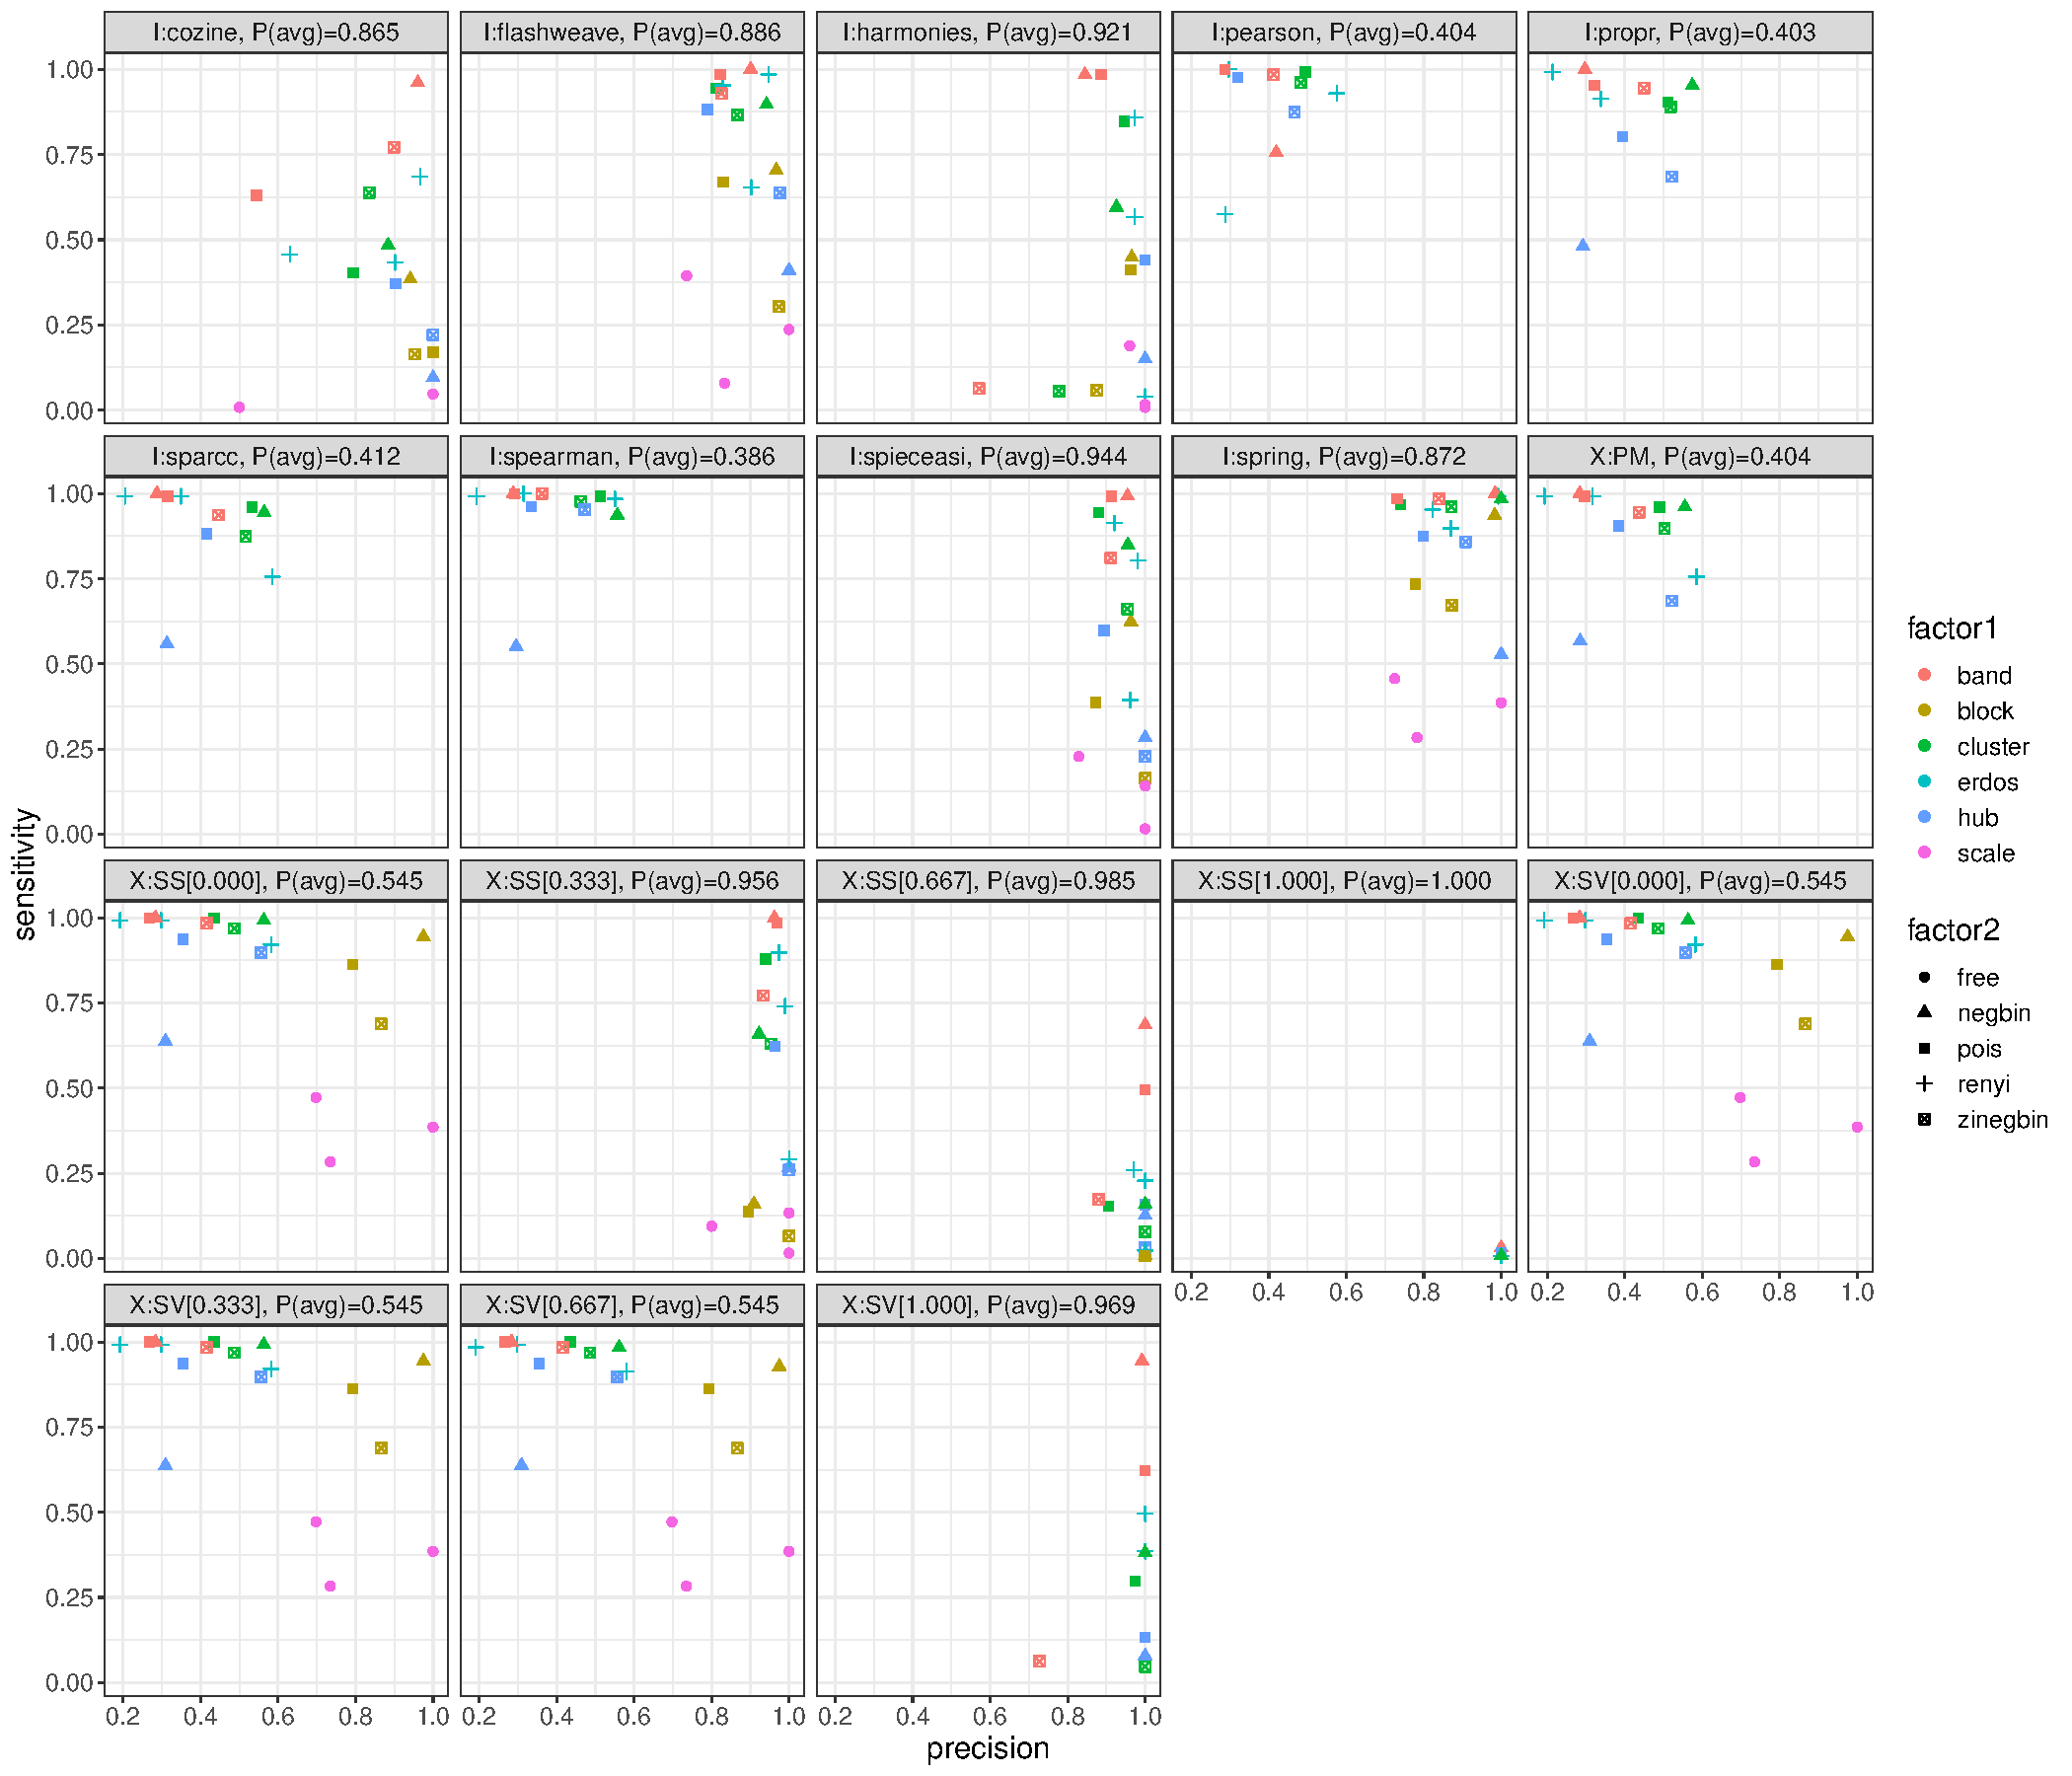
\includegraphics[width=0.85\linewidth]{figure5.pdf}
  \caption{
    \textbf{Networks generated using different network inference methods show notable differences both in terms of edge-density and connectivity}.
    \textbf{(A)} The six different networks generated by the different network inference methods are very dissimilar.
    The green links are positive associations and the orange links are negative associations.
    A threshold of 0.3 was set for the methods that infer pairwise correlations (\ac{sparcc}, Spearman, Pearson) and no threshold was set for the other methods.
    \textbf{(B)} The node overlap upset plot indicates that all the networks have a large number of common nodes involved in connections.
    Whereas, \textbf{(C)} The edge overlap upset plot shows that a very small fraction of these connections are actually shared.
  }
  \label{fig:figure5}
\end{figure}

\begin{figure}[h]
  \centering
  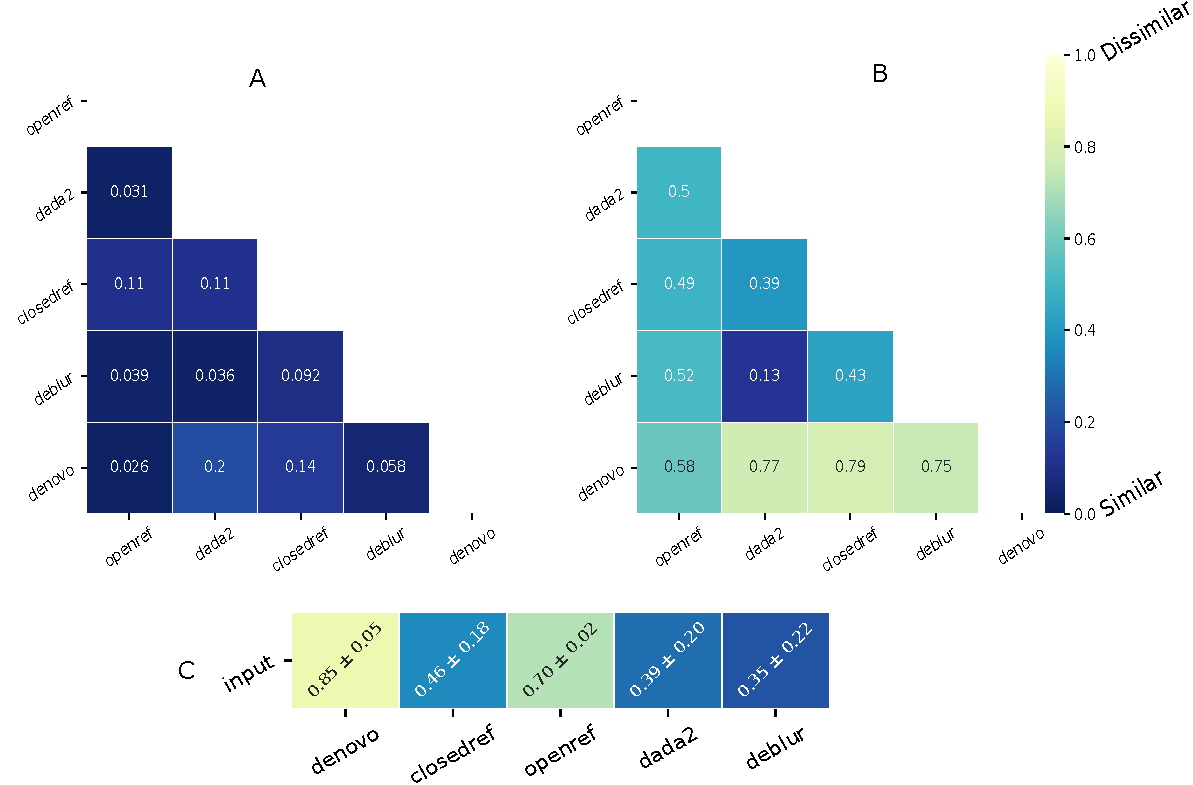
\includegraphics[width=0.9\linewidth]{figure6.pdf}
  \caption{
    \textbf{Network inference and taxonomic assignment have the highest influence on the inferred network structures.}
    \textbf{(A)} The network constructed using the default pipeline parameters (DC=\ac{dada2}, TA=\ac{ncbi}, OP=on, NI=\ac{sparcc}) is compared with networks generated when one of the steps use a different tool.
    The common connections (common with default) are in black, connections unique to the network are colored purple and connections in the default network and but not present in the current network are gray.
    \textbf{(B)} The L1 distance of the networks generated by changing one step of the default pipeline against the network generated using the default parameters.
  }
  \label{fig:figure6}
\end{figure}

\begin{figure}[h]
  \centering
  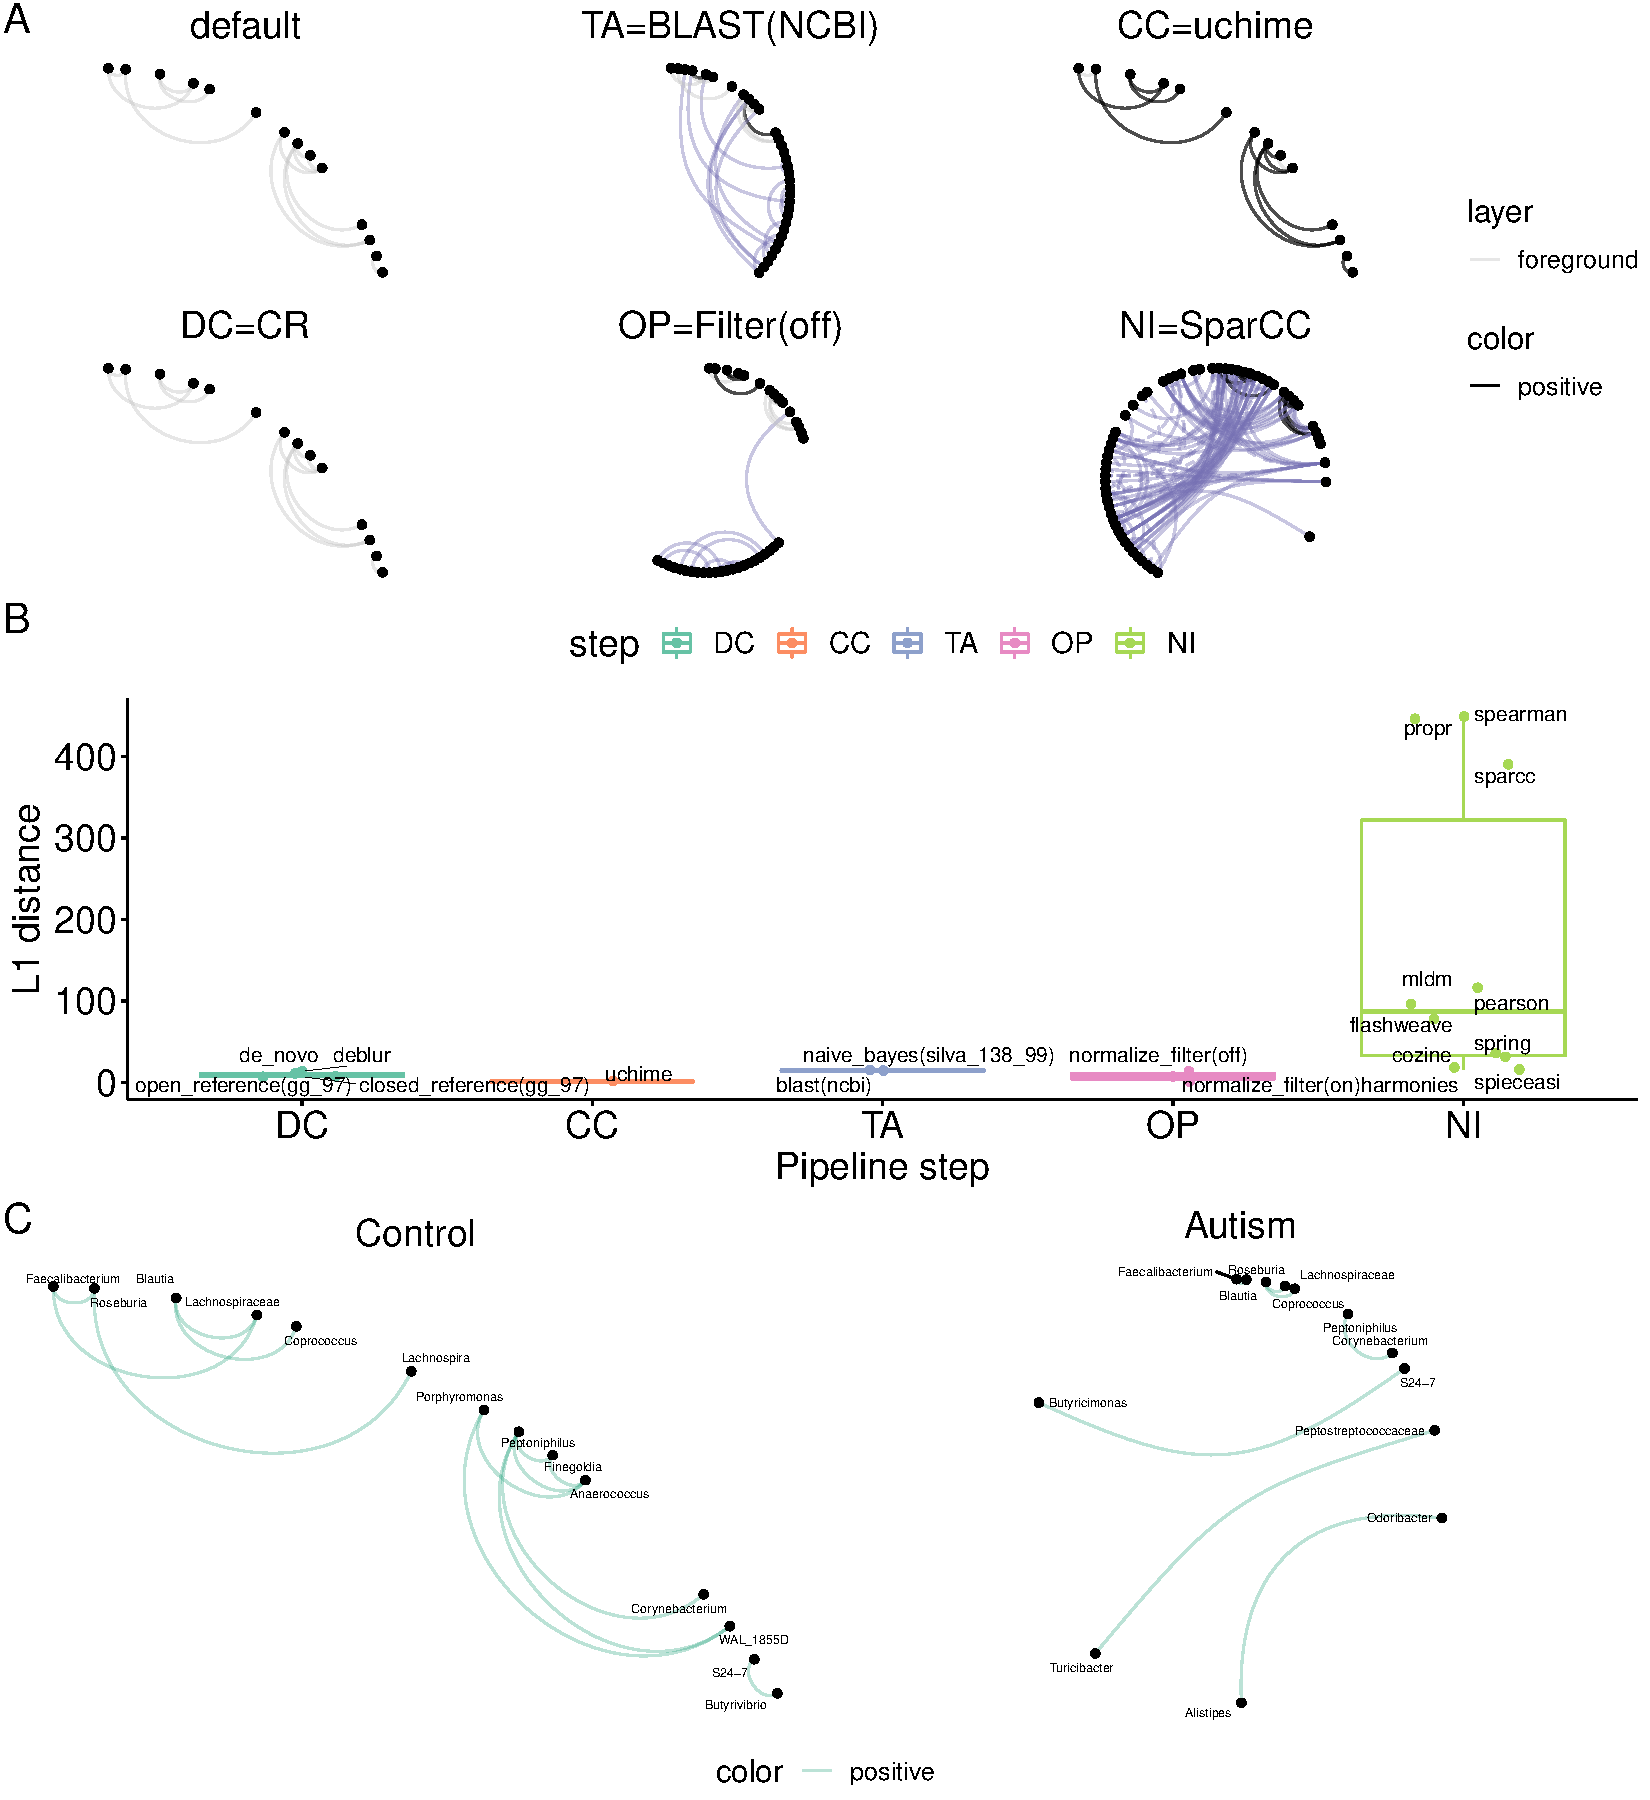
\includegraphics[width=17cm]{figure7.pdf}
  \caption{
    The consensus networks generated using the default pipeline settings for the Hard Palate \textbf{(A)} and Stool \textbf{(B)} body-sites.
}
  \label{fig:figure7}
\end{figure}


% \FloatBarrier

% \subsection*{Supplementary}%

% \setcounter{figure}{0}
% \renewcommand{\thefigure}{S\arabic{figure}}

% \begin{figure}[h]
%   \centering
%   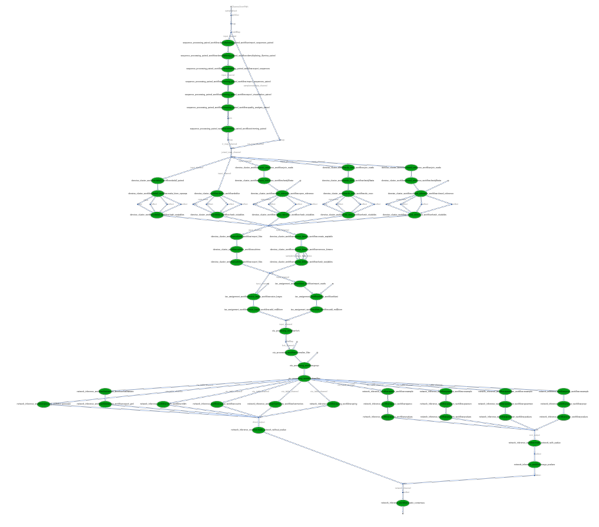
\includegraphics[width=0.67\linewidth]{figureS1.pdf}
%   \caption{
%     \textbf{Comparison of various denoising and clustering algorithms used in the pipeline}.
%     (A, B) Correlation of the abundances of the taxa that are common between the count matrices created by two different methods.
%     (A) The best correlation (most similar methods) is between open-reference and denovo.
%     (B) The worst correlation (least similar methods) is between open-reference and dada2.
%     (C) A heatmap showing the $\mathrm{R}^2$ of all pairwise comparisons of the methods.
%   }
%   \label{fig:figureS1}
% \end{figure}



% \begin{figure}[h]
%   \centering
%   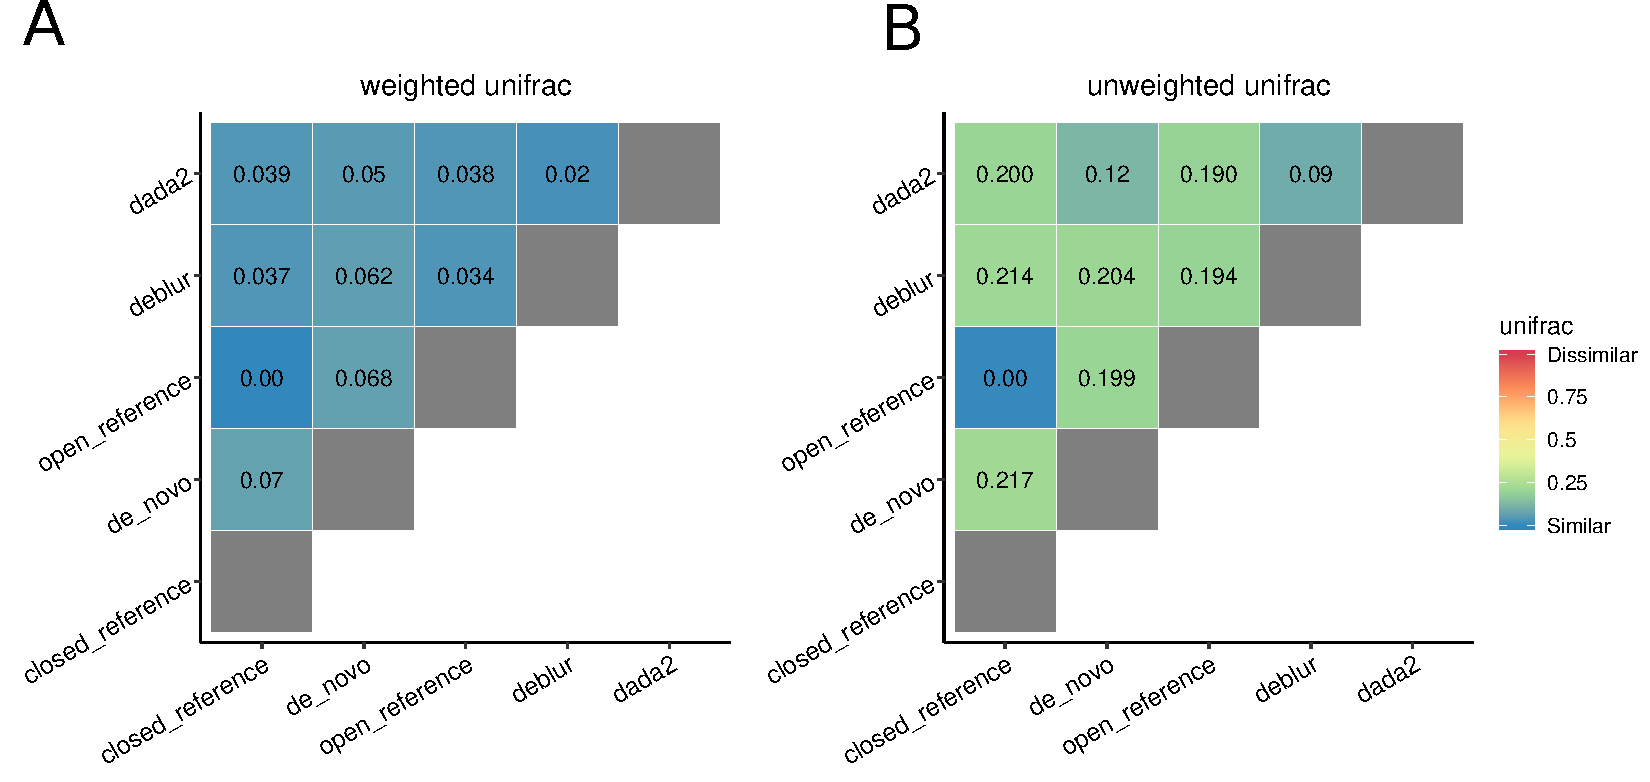
\includegraphics[width=0.8\linewidth]{figureS2.pdf}
%   \caption{Results of the mock community analysis. (A) Weighted unifrac (B) Unweighted unifrac}
%   \label{fig:figureS2}
% \end{figure}

% \begin{figure}[h]
%   \centering
%   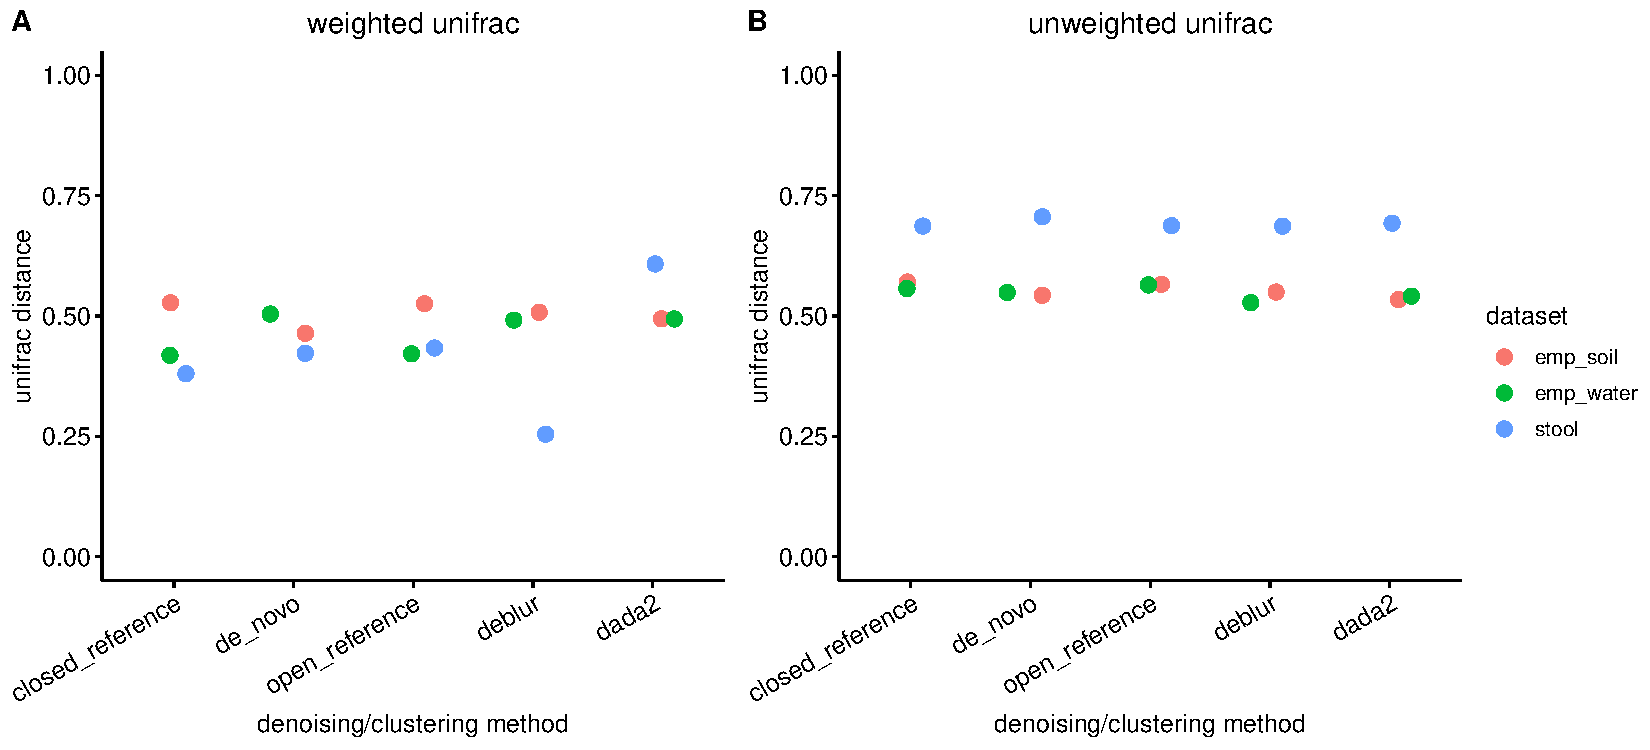
\includegraphics[width=0.8\linewidth]{figureS3.pdf}
%   \caption{Results of the synthetic community analysis. (A) Weighted unifrac (B) Unweighted unifrac}
%   \label{fig:figureS3}
% \end{figure}

% \begin{figure}[h]
%   \centering
%   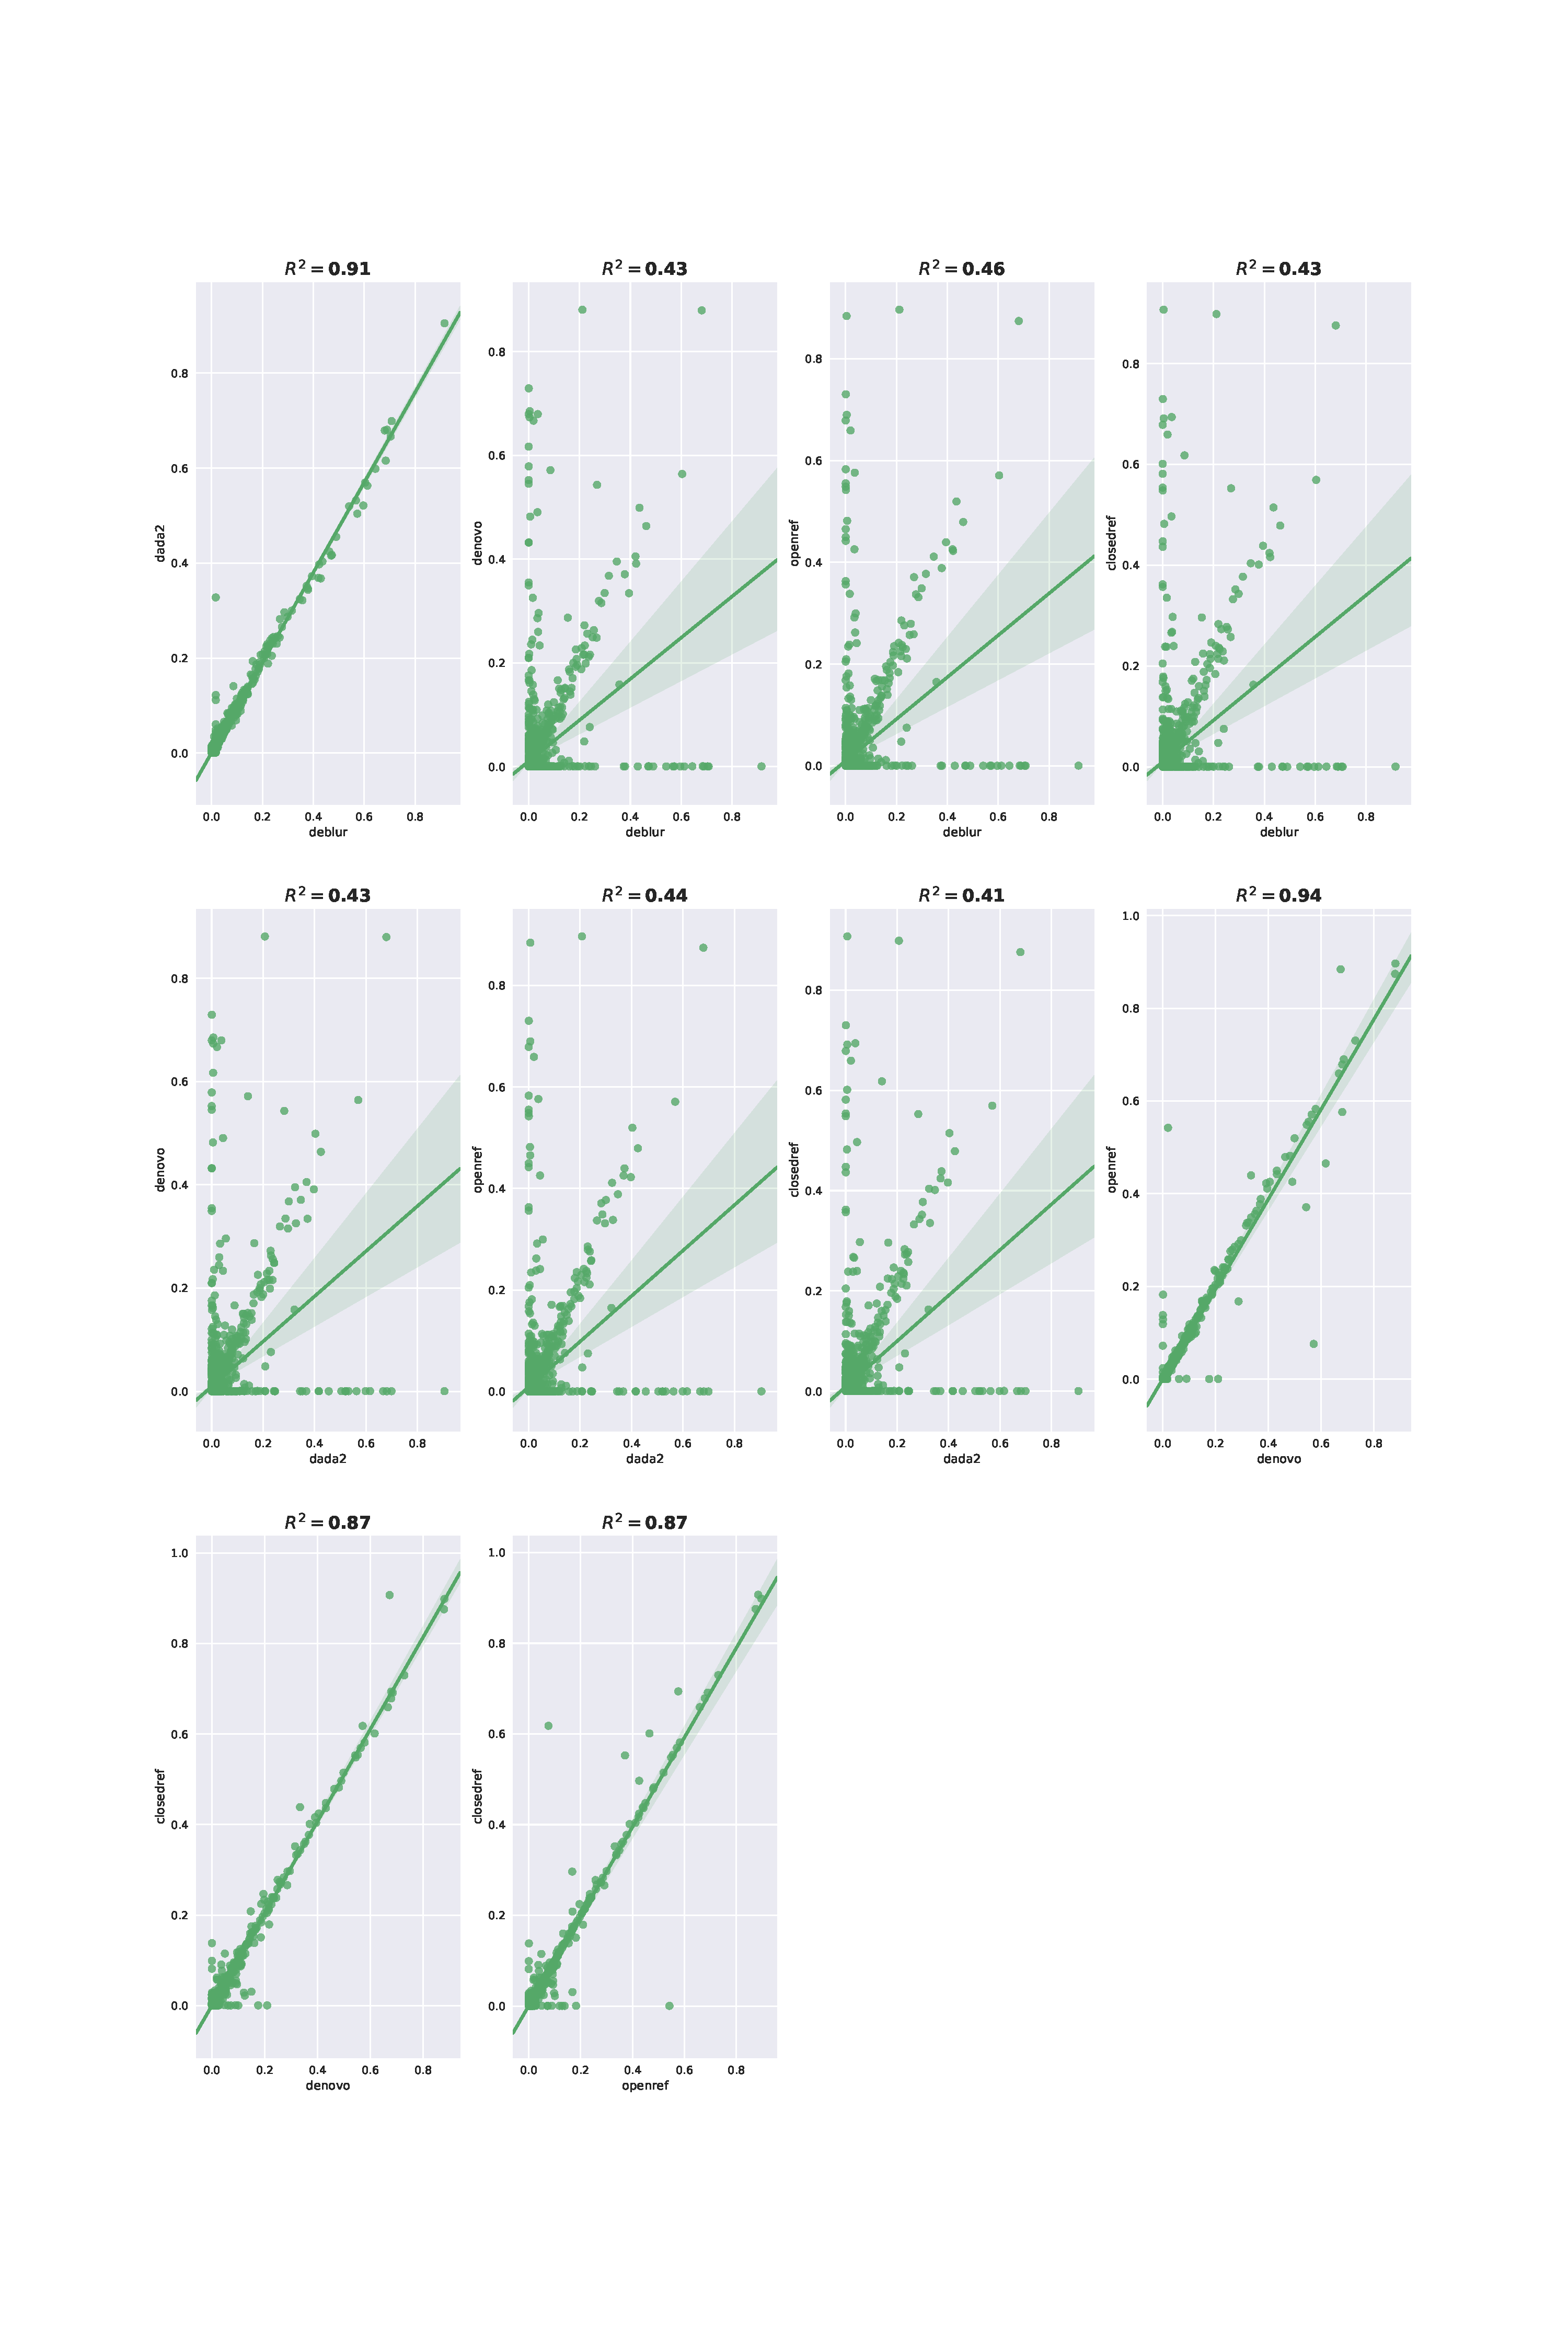
\includegraphics[width=0.8\linewidth]{pdf/all_denoise_reg.pdf}
%   \caption{All pairwise correlations comparing the similarity between different denoising and clustering methods}
%   \label{fig:figureS4}
% \end{figure}

% \begin{figure}[h]
%   \centering
%   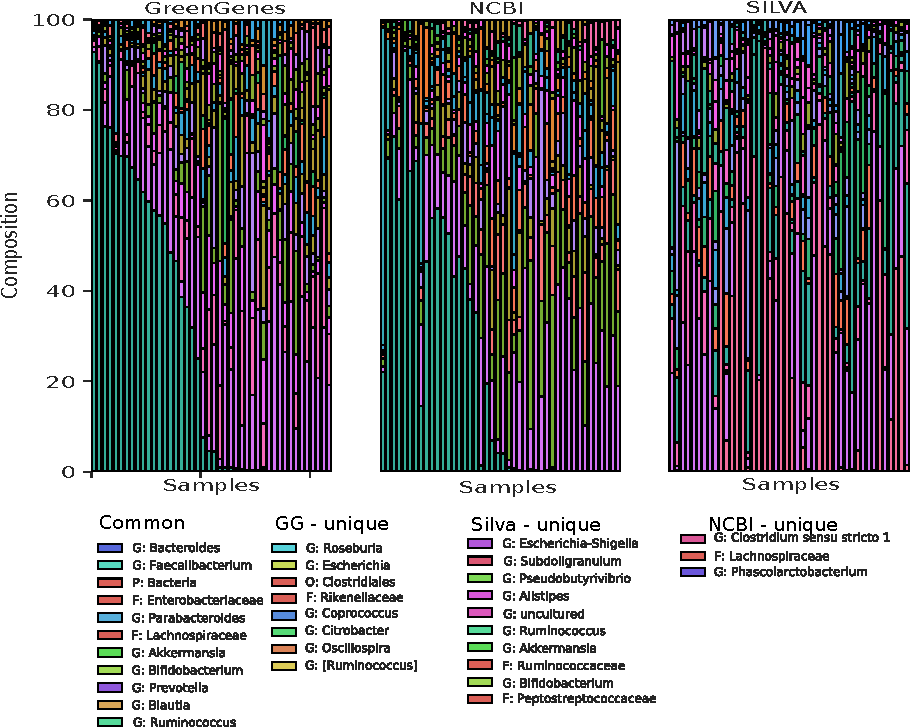
\includegraphics[width=\linewidth]{figureS4.pdf}
%   \caption{
%     \textbf{(A)} Taxonomy composition of the 20 most abundant genera predicted using different taxonomy references databases: Greengenes, SILVA and NCBI.
%     The legend shows the common and the unique genera among the taxonomy assignments.
% }
%   \label{fig:figureS4}
% \end{figure}

% \begin{figure}[h]
%   \centering
%   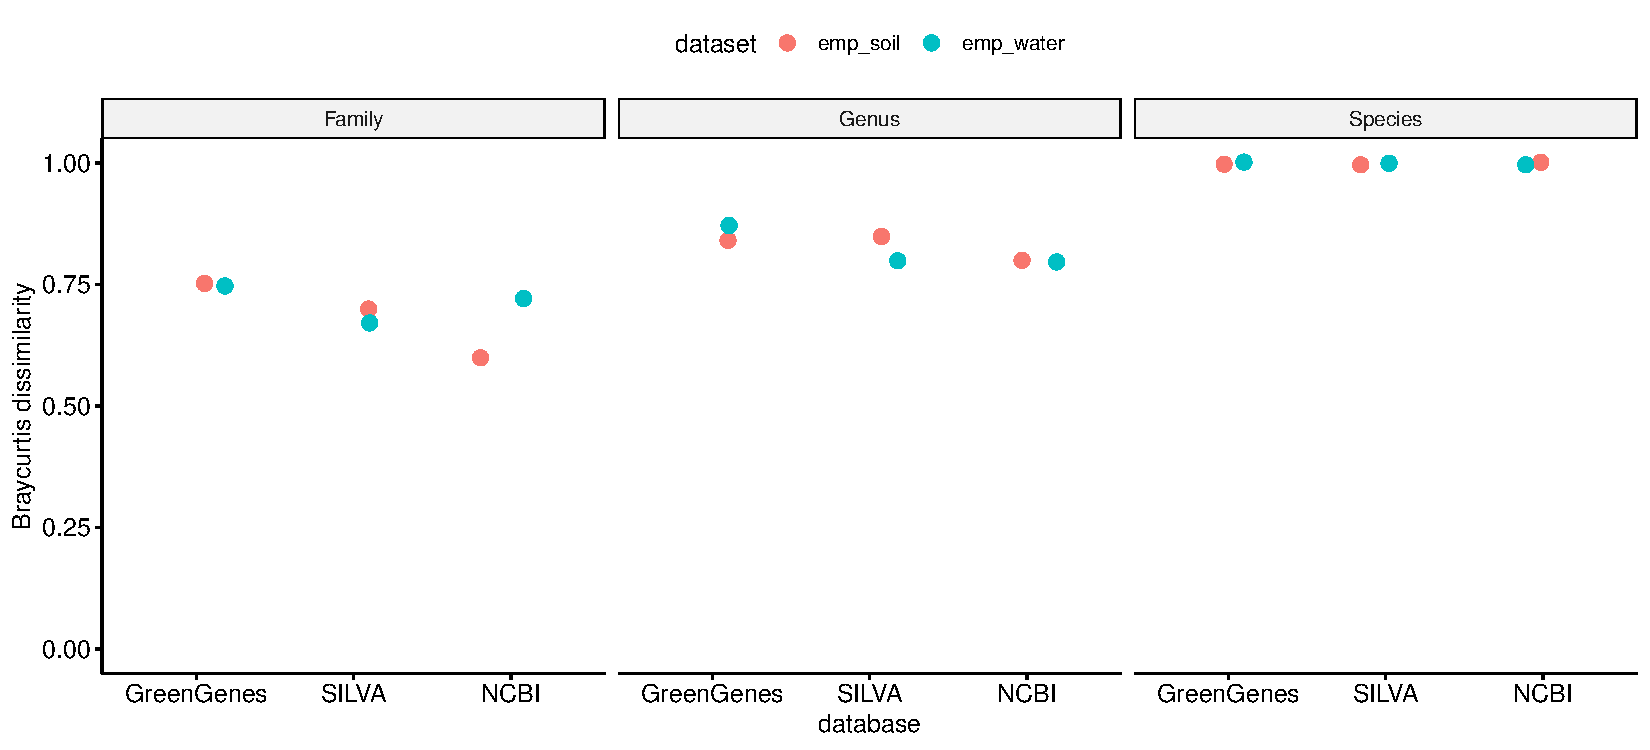
\includegraphics[width=\linewidth]{figureS5.pdf}
%   \caption{
%     The bray-curtis dissmilarity between the expected taxonomic composition and generated taxonomic composiion for the synthetic datasets.
% }
%   \label{fig:figureS4}
% \end{figure}

% \begin{figure}[h]
%   \centering
%   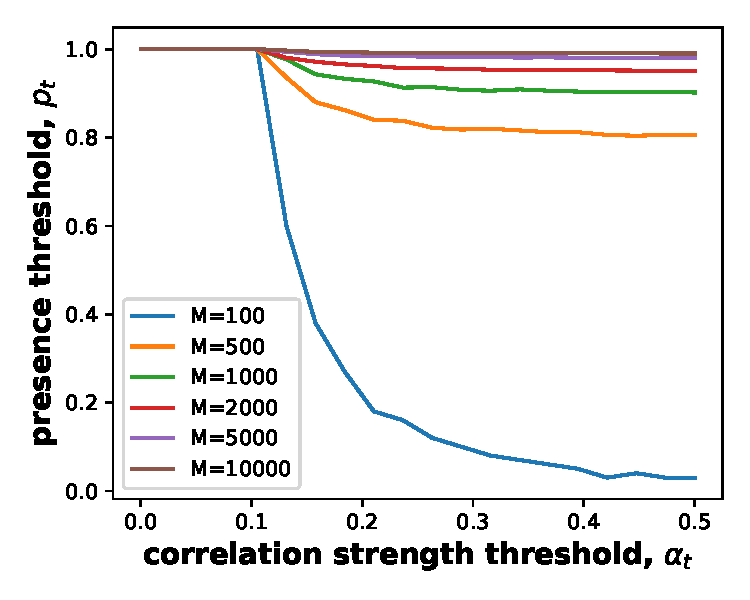
\includegraphics[width=\linewidth]{figureS6.pdf}
%   \caption{
%     The effect of OTU processing measurs on the OTU table
% }
%   \label{fig:figureS4}
% \end{figure}

% \begin{figure}[h]
%   \centering
%   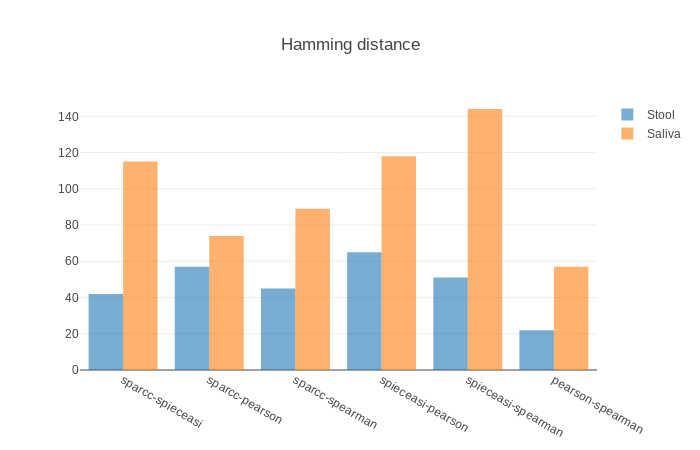
\includegraphics[width=0.8\linewidth]{png/hamming_distance.png}
%   \caption{The hamming distance between the networks is shown. The similarity between various methods was found to vary with the data-source used.}
%   \label{fig:figureS4}
% \end{figure}

% \begin{figure}[h]
%   \centering
%   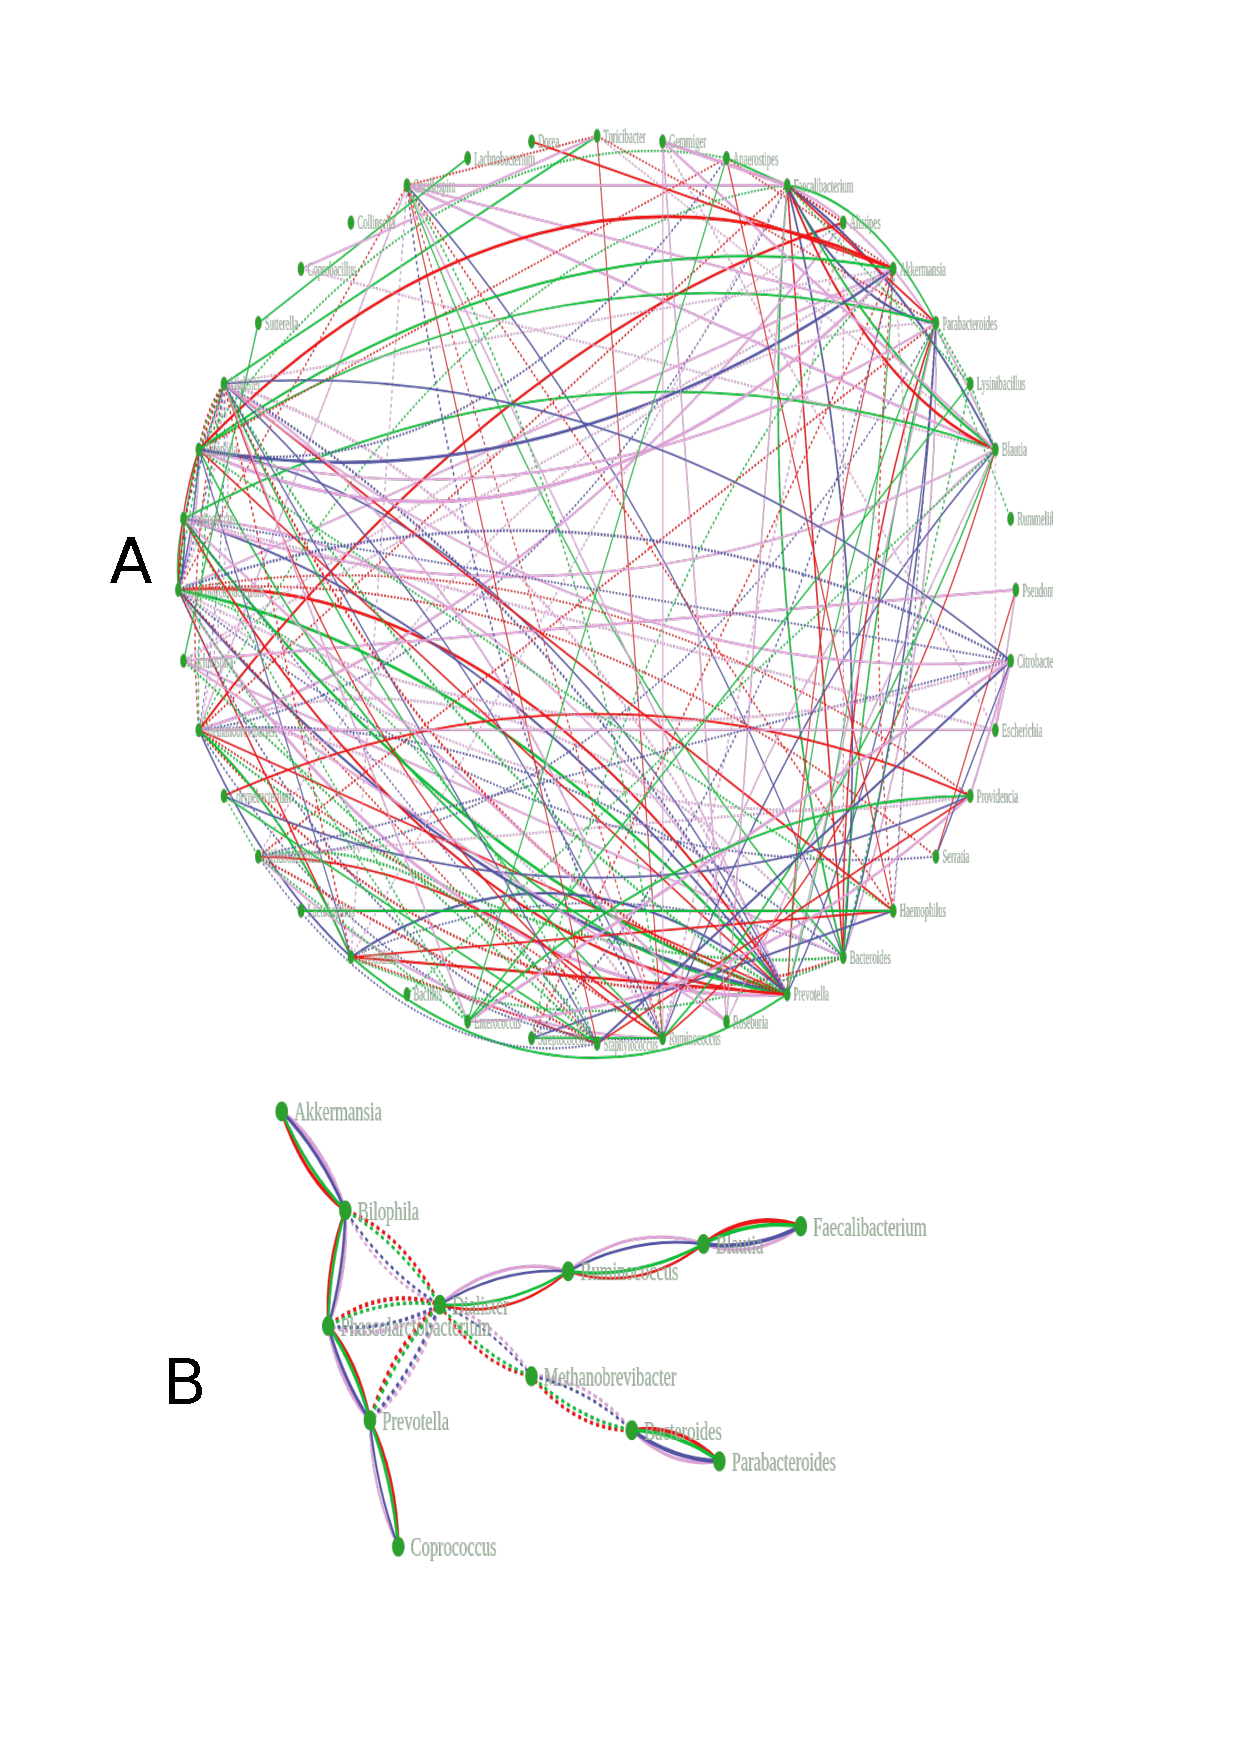
\includegraphics[width=0.8\linewidth]{pdf/denoise_network.pdf}
%   \caption{A network showing union and intersection of networks generated using certain combination of methods}
%   \label{fig:figureS5}
% \end{figure}


\end{document}
